\documentclass[a4paper]{article}
\usepackage[english]{babel}
\usepackage[utf8x]{inputenc}
% package for including graphics with figure-environment
\usepackage{graphicx}
\usepackage{hyperref}
\usepackage{float}
\usepackage{amssymb,stmaryrd}
% colors for hyperlinks
% colored borders (false) colored text (true)
\hypersetup{colorlinks=true,citecolor=black,filecolor=black,linkcolor=black,urlcolor=black}

% Commentbox package
\usepackage[most]{tcolorbox}
% Braket notation package
\usepackage{braket}

% package for bibliography
\usepackage[authoryear,round]{natbib}
% package for header
\usepackage[automark,headsepline]{scrlayer-scrpage}
\pagestyle{scrheadings}
\ihead[]{Meyer, Springer, Kawamura, Heidenreich}
\ohead[]{\today}
\cfoot[]{\pagemark} 

\begin{document}
	\title{
	\begin{figure}[!ht]
		% \flushleft
			
\includegraphics[width=0.26\textwidth]{img/THlogoheader.pdf}
	\end{figure}
	\vspace{1cm}
	\Huge Here you can insert the title of \\ your seminar paper \\
	}
	
	\vspace{1cm}
	
	% if you are the only author, you might use the following
	% \author{Name of student}	
	
	% Insert here your name and correct mail address
	\author{\Large \href{mailto:ben_konrad.meyer@smail.th-koeln.de@smail.th-koeln.de}{Ben Konrad Meyer} \and \Large \href{mailto:mike.springer@smail.th-koeln.de}{Mike Springer} \and \Large \href{mailto:kai.kawamura@smail.th-koeln.de}{Kai Kawamura} \and \Large \href{mailto:karl_julian.heidenreich@smail.th-koeln.de}{Julian Heidenreich} \\
	\vspace{1cm}}
	
	% name of the course and module
	\date{
	\large Modul: Verteilte Systeme \\ 
	\vspace{0.8cm}
	\large Lecturer: Name of the lecturer \\
	\vspace{1cm}
	\today
	}

	\maketitle
	\setlength{\parindent}{0pt}

\vspace{2cm}
\begin{abstract}
This template can be used for seminar papers. For more tips and tricks regarding the use of figures, tables, quotations, references, footnotes, enumerations, etc. please download the Masterthesis template. 

\end{abstract}
	\newpage
	\tableofcontents
	\newpage
\section{Introduction} \label{sec:introduction}
The goal of this paper is to explore the opportunities presented by quantum computing and its difficulties,
both in terms of information theoretical Aspects inherent to the concept and in practical aspects of its current
implementations.

Without first introducing the differences between a quantum computer and classical computer most Readers would however
lack the required context to understand the following paper and as such, this introduction will explain the most
critical aspects.

\subsection{Differences between classical and quantum computing theory} \label{subsec:diffclassquanttheory}
The first critical difference between the two computing methods in their theory is their most simple concept of data:
The classical computing theory operates on bits, a simple scalar value that is always one of a finite set of values
(typically either 1 or 0), with their only connection the one imposed by the algorithms in use.
It is also deterministic, with no true randomness, merely internal state that cannot be deduced from outside the system
and can be used to generate unpredictable, but not random values.

In contrast, quantum computing theory operates on the qubit, a superposition of 1 and 0 that is either of the values
with a given probability.
These qubits are typically either represented as a complex number or a unit vector.
Furthermore, for must practical application the qubits in use are not independent but entangled with some number of
other qubits, forming an entangled register, where the superpositions of the individual qubits are connected.
The probabilistic nature of qubits also gives quantum computing access to true randomness without any need for the
complex pseudo random number generators of classical computing.
Indeed, most quantum computing focuses on eliminating the randomness so that the odds of all correct results combined
come as close to 1 as possible, while the likelihood of the other results are reduced to near zero.

Another difference appears due to the physical requirements of superposition: All operations other than measurement on
a quantum computer must be reversible and copying an arbitrary register is impossible\ref{subsec:no-cloning}.
Neither of these restrictions appears for classical computers and as such while there are quantum algorithms where
quantum computers vastly outperform classical computers there are equally classical algorithms where quantum computers
are far less efficient than classical computers, though every classical algorithm has a quantum equivalent % TODO ref or citefor equivalence

\subsection{Practical differences between classical and quantum computers} \label{subsec:diffclassquantpracticey}
Not only are there inherent differences in the practical aspects between classical and quantum computers, there are also
differences induced by the fact that while classical computing has matured over the past decades, quantum computers are
still in the experimental phase.

One aspect where the two paradigms differ is scalability.
While it is possible to simply increase the number of gates of a classical computers, albeit perhaps sacrificing some
performance per gate and latency to heat dissipation concerns, to produce a more powerful classical computer a quantum
computer requires its system to remain in coherence\cite{find explaination}, which makes any scaling of the system a
complex tasks for physicists in addition to making simply connecting two quantum computers into one larger one impossible.

Another aspect is energy efficiency.
For a classical computer every single state needs a gate, whose operation comes with a small, but quickly compounding
cost in heat loss.
Indeed, heat dissipation concerns are the primary limiters for processor size.
While a quantum computer in theory also produces some waste heat per gate, its gates also operate on a superposition on
states and as such could theoretically be far more energy efficient.
In practice this advantage is however entirely counteracted by the fact that current quantum computers require extremely
low temperatures and as such spend most of their energy not on their actual operation, but on the cooling systems they
require to function.
Should a way to keep a quantum computer stable at room temperature be discovered however, quantum computers would easily
change from less to more energy efficient than classical computers.

The final problem that faces quantum computers that is largely solved by classical computers is error correction.
In a classical computer the occasional errors in gate operation, ironically due to quantum mechanical effects, is
corrected by duplicating the calculation and taking a majority vote of the result.
The no-cloning-theorem\ref{subsec:no-cloning} however prevents quantum computers from copying this approach instead
other algorithms have to be used to avoid the final practical superposition differing too much from the theoretical
superposition determined by the intended algorithm. % TODO ref to error correction chapter


\section{Der Kontrast zwischen Klassischen und Quantencomputern}

- Qubit vs Klassisches Bit

- Umkehrbare Operationen in QC

- Alle KC Operationen in QC möglich, aber teilweise komplexer

- QC kann Operationen machen, die der KC nicht kann (größtenteils Zufallselemente)

- Zwei Beispiele folgen, die das verdeutlichen

\subsection{No Cloning Theorem}

- Proof by Contradiction (Umkehrbare Operationen)

- Macht Klassische Error Correction unmöglich

\subsection{Verschränkte Teleportation}

- Braucht Setup (verschränktes Qubit teilen)

- überträgt einen Quantenzustand

- - Zustand am Ursprung wird zerstört (no cloning theorem)

\section{Quantenhardware}
\label{sec:quantenhardware}

Die Realisierung eines Quantencomputers ist durch hohe technische herausforderungen geprägt. Um die besonderen Eigenschaften der Qubits eines Quantencomputers, wie Superposition und Verschränkung, nutzen zu können, müssen sie durch externe Einflüsse geschützt werden und die Dekoheränz minimiert werden.
Äußere Einflüsse wie Temperaturschwankungen, elektromagnetische Felder oder Strahlung aller Art können die Qubits beeinflussen. Aus diesem Grund werden Quantencomputer bei extrem niedrigen Temperaturen und in einem Vakuum betrieben.\\

Außerdem ist nicht nur die Herstellung der Qubits eine Herausforderung, sondern auch die Steuerung, Auslesung und Korrektheit von physikalischen Qubits.

\subsection{Dekohärenz}
\label{sub:dekohaerenz}
Dekoheränz ist ein zentrales Konzept, welches wichtig in der Entwicklung von Quantencomputern ist. Der Prozess der Dekoheränz beschreibt den Verlust der koheränten Quanteneigentschaften eines Qubits durch Wechselwirkung mit der Umgebung.
Diese Veränderung führt zu einem Übergang von quantenmechanischem Verhalten zu einem klassischem Verhalten von Bits.\\

In der Quantenmechanik können Systeme in Überlagerungszuständen existieren, wobei mehrere Zustände gleichzeitig eingenommen werden können. Diese Eigenschaft erklärt auch das Phänomen der Quanteninterferenz.
Äußere Einflüsse durch die Umgebung kann eine Verschränkung von Qubits zerstören. Dies führt dazu, dass die Phasenbeziehungen zwischen den Qubits beeinflusst oder gar aufgehoben werden.
Folgernd verliert das System die Interferenzeffekte und verhält sich zunehmend klassischer. Diese Zeit nennt man Dekoheränzzeit.\\

Die \textbf{Dekoheränzzeit} ($T_2$) eines Qubits misst die Länge der Zeit, in der er in der Lage bleibt kohärent zu bleiben, welcher danach von äußeren Einflüssen zerstört wird.
Neben $T_2$ wird auch häufig die \textbf{Relaxationszeit} ($T_1$) gemessen, welche angibt, wie lange ein Qbit im angeregten Zustand bleibt, bevor es auf sein Grundzustand zurückfällt.
In der Realität ist die Dekoheränzzeit jedoch in den meisten Fällen kürzer als die Relaxationszeit.\\

\textbf{Berechnung der Dekoheränzzeit}\\
Durch eine Messung der zeitlichen Abnahme der Koheränz eines beispielhaften Qubits kann die Dekoheränzzeit eines Systems festgelegt werden.
Bei einem Quantencomputer, der auf dem Spin eines Teilchen beruht, kann dies durch die \textbf{Spin-Echo-Methode} gemessen werden.
Quantencomputer, die auf anderen Qubits basieren, haben equivalente Methoden um die Kohärenz zu messen.\\

Das einfachste Modell zur Beschreibung der Dekoheränzzeit ist die \textbf{Exponentielle Abnahme der Kohärenz}

\begin{equation}
    C(t) = C(0)*e^{-t/T_2}
\end{equation}

Dabei ist:\\
$C(t)$ Die Kohärenz des Qubits zum Zeitpunkt t\\
$C(0)$ Die initiale Koheränz\\
$T_2$ Die Dekoheränzzeit\\

Indem man den Kohärenzverlust experimentell misst und die Werte in eine exponentielle Abklingfunktion einpasst, erhält man $T_2$\\

\begin{tcolorbox}[title=Kommentar,
    title filled=false,
    colback=cyan!5!white,
    colframe=cyan!75!black]
    Die \textbf{Dekoheränzzeit} kann auch durch genauere jedoch auch deutlich kompliziertere weise errechnet werden.
    Bekannte Methoden hierfür wären zum Beispiel die Spektrale Analyse, Dynamische Entkopplung, Hahn-Echo und Ramsey-Interferometrie.
    Außerdem wird duch das häufige messen der Dekoheränzzeit diese indirekt verlänger. Diesen Effekt nennt man Quanten-Zeno-Effekt.\\
    Zuletzt muss auch die Lindblad-Gleichung genannt werden welche den Zeitverlauf der Dichtematrix in einem Offenen Quantensystem beschreibt.
    \begin{equation}
        \frac{dp}{dt} = -i[H,p]+\sum_i(L_ipL^\dagger_i-\frac{1}{2}\{L^\dagger_i L_i,p\})
    \end{equation}
    Diese Themen sprengen jedoch den Rahmen dieser Arbeit in Richtung Physik und werden deswegen nicht weiter behandelt.
\end{tcolorbox}

\subsection{Universelle Quantencomputer}
\label{sub:universelle_quantencomputer}
Universelle Quantencomputer beruhen grundlegend auf einem Gatter Modell, wie bereits in diesem Artikel beschrieben. Folgend sind drei der meist erforschten
Methoden, welche dieses Modell physikalisch umsetzen.\\

Ein prominentes Beispiel für die Umsetzung eines universellen Quantencomputers ist der \textbf{Sycamore Chip}, welcher auf supraleitenden Qubits basiert.
Dieser Chip ist in einem Gatter angeordnet für die Kommunikation zwischen Qubits und die durchführung von Quantenoperationen.\\

\begin{figure}[H]
    \centering
    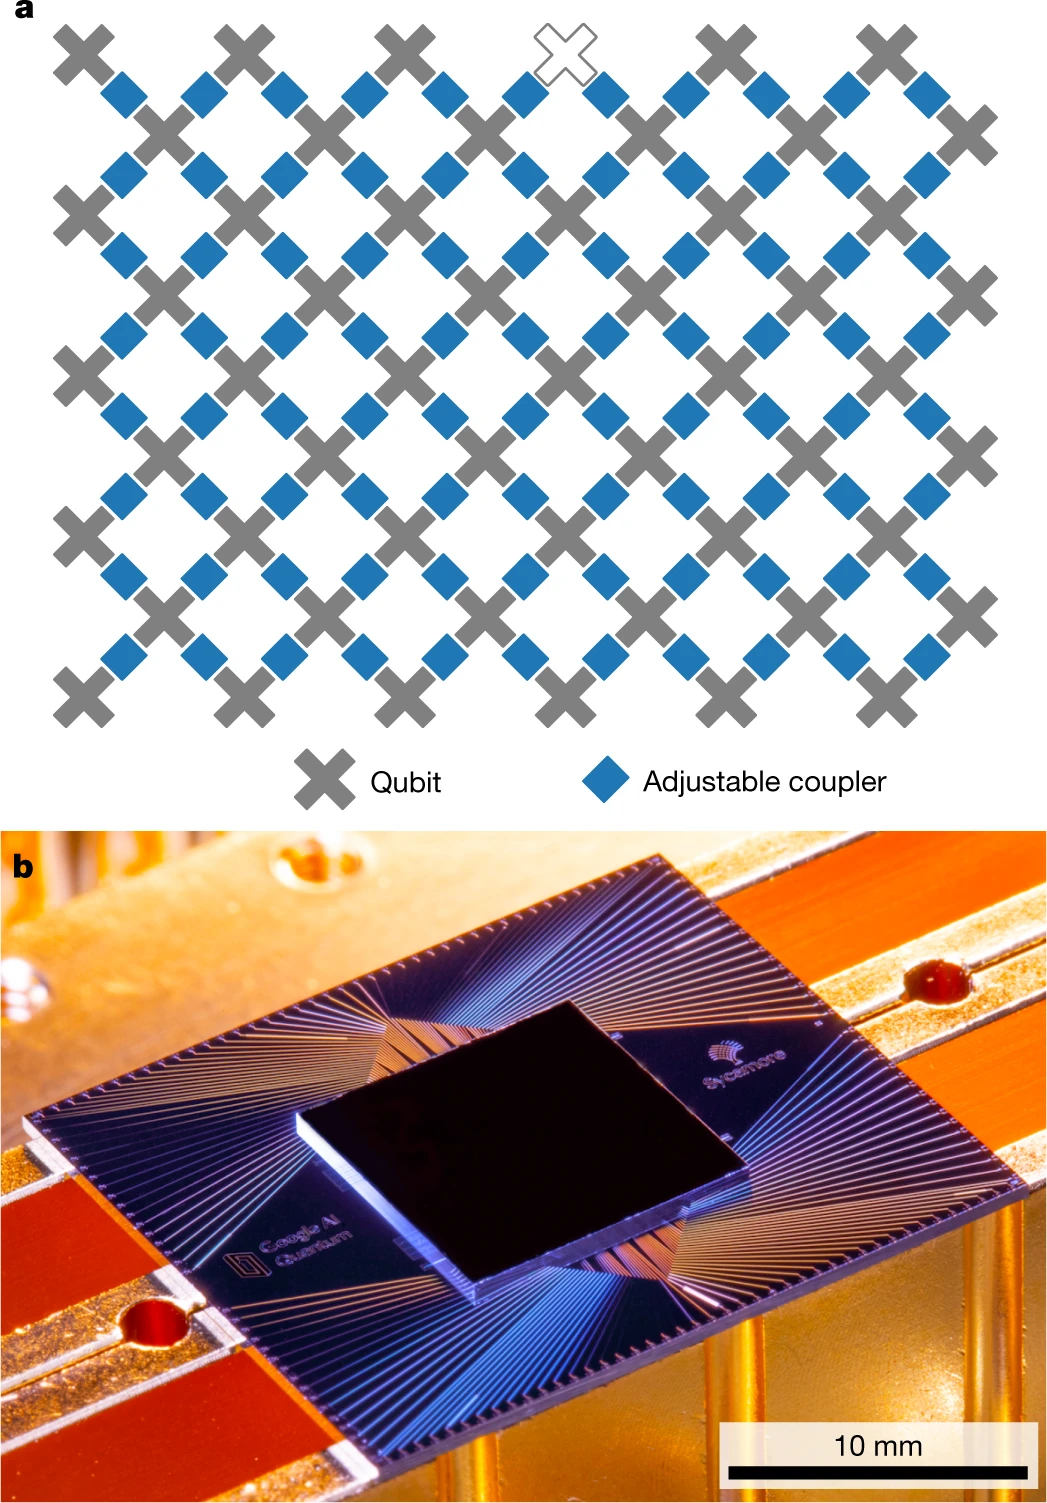
\includegraphics[width=0.7\linewidth]{img/SycamoreChip.png}
    \caption{Sycamore Chip von Google}
    \label{fig:Sycamore}
\end{figure}

\subsubsection{Supraleitende Qubits}
\label{subsub:superleiter}
Quantencomputer mit Supraleitern funktionieren mit elektrischen Schaltkreisen, die bei Temperaturen nahe dem absoluten Nullpunkt betrieben werden. Solche Temperaturen sind nötig,
um die supraleitende Eigenschaft aufrecht zu erhalten.\\

Zwei häufig benutze Qubit-Typen dieser elektrischen Schaltkreise sind:\\
\textbf{Transmon-Qubits}, basiert auf der Ladung des Energieniveaus, welche durch eine Josephson-Junktion kontrolliert wird.\\
\textbf{Flux-Qubits} werden auch durch Josephson-Junktions kontrolliert, beruhen jedoch auf dem magnetischen Fluss in der Schleife.\\

Beide Ansätze basieren auf dem \textbf{Josephson-Effekt}, welcher auftritt, wenn ein supraleitender Strom durch eine dünne Isolierschicht zwischen zwei Supraleitern fließt.\\
Dieser Effekt hat zur Folge, dass eine nichtlineare Spannung-Stom-Beziehung entsteht und für die Manipulation von Qubits genutzt wird.\\

\begin{figure}[H]
    \centering
    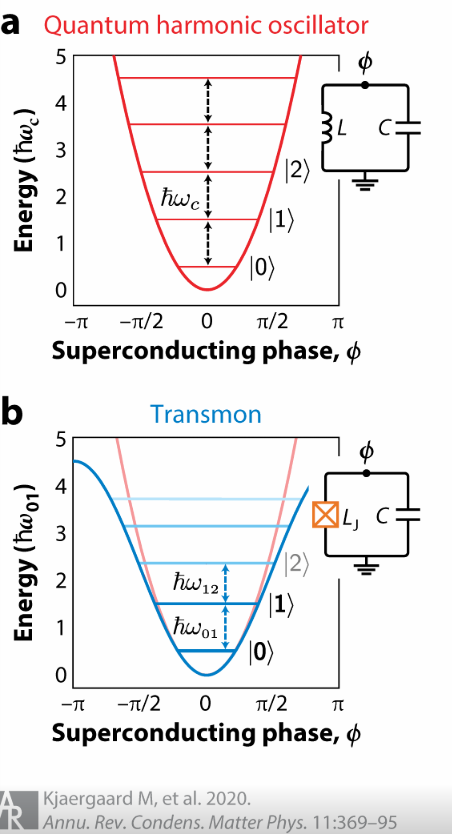
\includegraphics[width=0.75\linewidth]{img/JJ.png}
    \caption{Josephson-Effekt mit einem Josephson Junktion}
    \label{fig:Josephson-junktion}
\end{figure}

In der vorliegenden Abbildung wird der Unterschied zwischen einer harmonischen Quantenschwankung (a) und der nichtlinearen Schwankung des Energie Niveaus der Josephson Junktion (b) abgebildet.\\

Der Phasenunterschied bei der harmonischen Oscellation, gekennzeichnet als $\hbar\omega_c$, ist identisch. Auf der Abbildung ist zu sehen, dass das Energieniveau der Phasen zwischen $\ket{0} \leftrightarrow \ket{1}$
und $\ket{1} \leftrightarrow \ket{2}$ identisch ist und dadurch nicht unterschieden werden kann zwischen welcher Phase gewechselt wurde.\\

Mit einer Josephson Junktion kann jedoch eine nichtlineare Schwankung des Energieniveaus erreicht werden, die auf der Abbildung als orangenes $\boxtimes$ gekennzeichnet ist (b).
Durch diese nichtlineare Schwankung ist das Energie Niveau zwischen den Phasen $\ket{0} \leftrightarrow \ket{1}$ und $\ket{1} \leftrightarrow \ket{2}$ unterschiedlich groß und kann somit unterschieden werden.
Der als $\hbar\omega_{01}$ gekennzeichnete Energieunterschied ist unser Qubit\\

\textbf{Steuerung und Auslesung}\\
Die Steuerung der Josephson-Junktion erfolgt durch Mikrowellenpulse, welche die Energie des Qubits verändern. Die Auslesung erfolgt durch eine Mikrowellenresonanz um die Energie des Qubits zu messen.\\

\subsubsection{Quantenpunkte}
\label{subsub:quantenpunkte}
Quantencomputer basierend auf Quantenpunkten, auch Quantum-Dot genannt, nutzen winzige Halbleiterstrukturen um Qubits zu realisieren.
Quantum-Dots sind künstlich erzeugte Nano-Partikel, in denen Elektronen in drei Dimensionen eingeschlossen sind, was zu quantisierten Einergiezuständen führt.\\

Die Größe eines Quantum-Dots ist typischerweise 2-10 Nanometer und es schließt eine kleine Anzahl oder ein einzelnes Elektron ein.
Für die Fertigung werden oftmals Galliumarsenid (GaAs) oder Silizium (Si) verwendet. Der physikalische Einschluss der Elektronen schränkt ihre
Bewegung stark ein, wodurch ein quantisiertes Energieniveau entsteht. Dies ähnelt dem Energieniveaus eines Atoms, weswegen Quantum-Dots auch als künstliche Atome bezeichnet werden.\\

Die Zustände der Qubits werden durch die Eigenschaften einzelner Elektronen in den Quantum Dots definiert. Es gibt zwei Hauptansätze zur Realisierung von Qubits mit Quantum Dots.\\

\textbf{Ladungs-Qubits}\\
Der Ladungszustand eine Quantum Dots kann als Qubit verwendet werden. Die Ladung eines Elektrons kann entweder 0 oder 1 sein, was als $\ket{0}$ und $\ket{1}$ interpretiert wird.
Für eine Messung wird der Ladungszustand mit einer Kapazitätsmessung der Tunnelströme ermittelt.
Für die Manipulation des Qubits werden elektrische Felder verwendet, um die Elektronen in den Quantum Dots zu bewegen.\\

Diese Methode ist durch die Ladungsquantisierung sehr genau, jedoch auch sehr empfindlich gegenüber Störungen durch die Umgebung.\\

\textbf{Spin-Qubits}\\
Die Spin-Eigenschaften von Elektronen in Quantum Dots können auch als Qubit verwendet werden. Hierbei sind die beiden Spinrichtungen($\uparrow$ für Spin-Up und $\downarrow$ für Spin-Down)
dieser beiden Spinrichtungen entsprechen den Zuständen $\ket{0}$ und $\ket{1}$. Und die Kombination aus beiden Zuständen ergibt eine Superposition.\\

\begin{figure}[H]
    \centering
    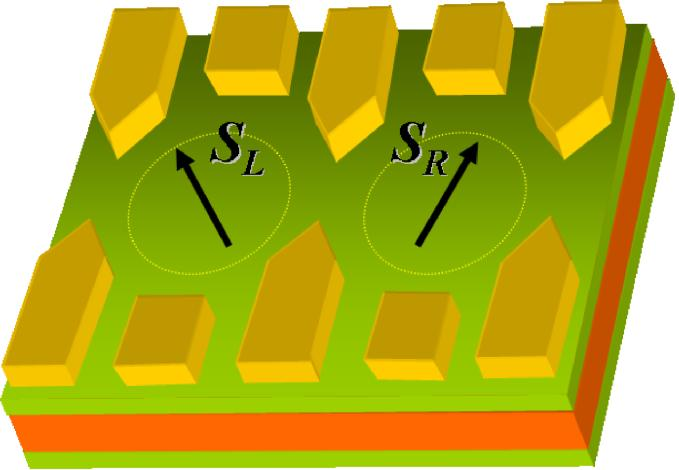
\includegraphics[width=0.75\linewidth]{img/QD.png}
    \caption{Ein doppel Quantum-Dot Qubit}
    \label{fig:double-Quantum-Dot}
\end{figure}

In der Abbildung ist ein Doppel Quantum-Dot Qubit dargestellt. Sowohl in $S_L$ als auch $S_R$ befinden sich Elektornen. Beide können seperat voneinander, sowohl im Spin als auch Ladung, manipuliert werden.
Durch die physikalische Nähe der beiden Quantum-Dots können durch Tunnelkopplung und Austauschwechselwirkung die beiden Qubits miteinander verschränkt werden.\\

Die Umsetzung dieser Methode beschränkt sich hauptsächlich auf die Spin-Variante. Der Grund dafür ist, dass durch die hohe Ladungsanforderung der Ladungsvariante die Qubits sehr empfindlich gegenüber Störungen sind.
Außerdem sind die Nachteile der Spin-Variante gegenüber der Ladungsvariante nicht so gravierend.\\
Jedoch sind die größten Herausforderungen die Herstellung der Halbleiterstrukturen und die Kontrolle der Elektronen in den Quantum-Dots.
Damit ist der größte Vorteil, die hohe Skalierbarkeit, auch der größte Nachteil, da die Herstellung und Kontrolle von vielen Quantum-Dots sehr aufwendig und schwierig ist.\\

\subsubsection{Topologische Quantencomputer}
\label{subsub:topologische_quantencomputer}
Der Ansatz von topologischen Quantencomputern ist völlig anders als die bisher genannten. Im Gegensatz zu verher erläuterten Quantencomputern, welche auf Eigenschaften einzelner Elektronen oder Energieniveaus basieren, basieren topologische Quantencomputer auf topologischen Eigenschaften von Materie.\\
Diese Methode soll das Problem der Dekoheränz minimieren, indem sie Qubits aus Majorana-Partikeln aufbauen.\\

\textbf{Topologie in der Physik}\\
In einem physikalischem System beschreibt die Topologie die Eigenschaften, welche sich nicht durch Deformation verändern lassen.
Ein Beispiel hierfür ist ein Kaffeebecher, der sich durch Verformung in eine Donutform umwandeln lässt. Beide haben die topologische Eigenschaft eines Loches.
Daraus folgernd ist es nicht möglich, einen Kaffeebecher oder ein Donut in eine Kugel zu verformen ohne die topologische Eigenschaft zu verändern.\\

\textbf{Funktionsweise}\\
Die physikalische Grundlage für topologische Quantencomputer liegt in speziellen Materialien und Systemen, die topologische Materiephasen unterstützen.
Ein prominentes Beispiel ist die Verwendung von Majorana-Quasiteilchen, die in bestimmten Supraleitern auftreten können.\\

\begin{figure}[H]
    \centering
    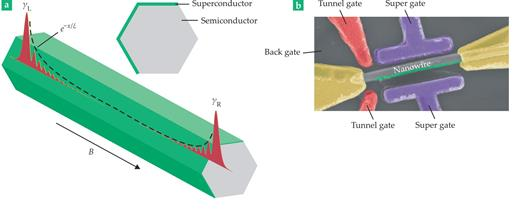
\includegraphics[width=0.75\linewidth]{img/Majorana.png}
    \caption{Nanowire mit Majorana-Quasiteilchen}
    \label{fig:Majorana}
\end{figure}

In der Abbildung ist ein Nanowire dargestellt, der durch ein Supraleiter und ein Magnetfeld in eine topologische Phase gebracht wird.
Diese Art von Partikel treten immer als Paar auf und bilden eine Art Brücke zwischen den Enden des Nanowire und besteht auf einer Vielzahl von Elektronen.
Diese Brücke wird durch die topologischen Eigenschaften der Majorana-Partikel stabilisiert und ist somit weniger anfällig gegenüber Störungen.\\


\begin{tcolorbox}[title=Kommentar,
    title filled=false,
    colback=cyan!5!white,
    colframe=cyan!75!black]
    Die Vertiefung der durch den Quanten-Hall Effekt entsteht wird nur oberflächlich behandelt. Ist jedoch essentiell für die Funktionsweise von Topologischen Quantencomputern.
\end{tcolorbox}

\textbf{Verpflechtung}\\
Braiding ist der Prozess, bei dem die Majorana-Partikel miteinander verflochten werden, um die Quantenbits zu manipulieren. 
Dies passiert auf einer zweidimensionalen Oberfläche, auf der die Majorana-Partikel miteinander verflochten werden.\\

\begin{figure}[H]
    \centering
    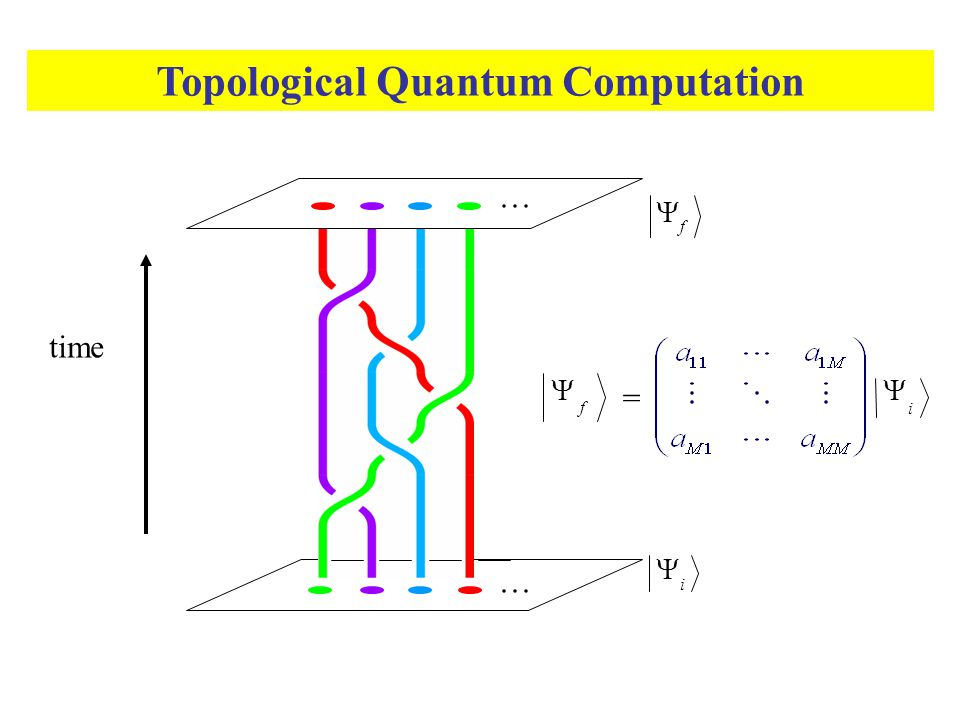
\includegraphics[width=0.75\linewidth]{img/TQC.png}
    \caption{Braiding von Majorana-Quasiteilchen}
    \label{fig:Braiding}
\end{figure}

Hierbei ist die Reihenfolge sehr wichtig, da durch diese Reihenfolge Quantenoperationen realisiert werden.
Jede Verpflechtung entspricht einer Quantenoperation und durch die Kombination von mehreren Verpflechtungen können beliebige Quantenoperationen realisiert werden.\\

Da die Informationen und Quantenoperationen in der Topologie steckt, sind sie gegenüber kleinen Fehlern in der Bewegung/Störungen unempfindlich.\\

\begin{tcolorbox}[title=Kommentar,
    title filled=false,
    colback=cyan!5!white,
    colframe=cyan!75!black]
    Die Technische Umsetzung von topologischen Quantencomputern ist deutlich komplizierter als es in diesem Abschnitt oberflächlich beschrieben ist.\\
    Bisher hat nur Google einen topologischen Quantencomputer vorgestellt, der jedoch noch nicht in der Lage ist, Quantenoperationen durchzuführen.
\end{tcolorbox}

\subsection{Quantum Error Correction}
\label{sub:quantum_error_correction}
Quantum Error Correction, oder auch QEC genannt, ist grundlegend wichtig für die funktionellen Betrieb eines Quantencomputers. Wie bereits in den vorherigen Abschnitten beschrieben,
sind Qubits sehr anfällig gegenüber Dekoheränz und Quantenrauschen.\\

\textbf{Warum ist Fehlerkorrektur notwendig}\\
Es ist unabdingbar, dass eine Fehlerkorrektur in Quantencomputern implementiert wird, da die Fehleranfälligkeit von physischen Qubits durch bessere Herstellung nur einen gewissen Grad an Fehlertoleranz aufbringen kann, welche nicht genug ist.\\

Fehler treten in Quantencomputer durch drei Hauptquellen auf.\\
1. \textbf{Dekoheränz:} Äußere Einflüsse wie Temperaturschwankungen oder elektromagnetische Felder zerstören die koheränten Eigenschaften der Qubits.\\
2. \textbf{Phasen-Flip-Fehler:} Die Phasenwinkel zwischen den Quantenzuständen werden verändert($\ket{0}\rightarrow\ket{0},\ket{1}\rightarrow-\ket{1}$).\\ 
3. \textbf{Bit-Flip-Fehler:} Die Zustände der Qubits werden verändert ($\ket{0}\rightarrow\ket{1},\ket{1}\rightarrow\ket{0}$).\\

Bei der Fehlerkorrektur von Quantencomputern ist jedoch zu beachten, dass diese nicht wie bei herkömmlichen Computern da durch das No-Cloning-Theorem keine Quanteninformationen kopiert werden können.\\

\textbf{Grundprinzip}\\
Quanten-Fehlerkorrektur verwendet \textbf{Redundanz} um Fehler zu detektieren und zu korrigieren, ohne das die eigentliche Quanteninformationen direkt ausgelesen werden.\\

Eine Art der Redundanz ist der Steane-Code, welcher auf 7 Qubits basiert. Dieser Zusammenschluss aus 7 Physischen Qubits bildet ein logisches Qubit,
welches maximal einen Fehler auf einem der 7 Qubits korrigieren kann. Treten jedoch mehrere Fehler auf, kann der Steane-Code diese nicht mehr korrigieren.\\

\begin{figure}[H]
    \centering
    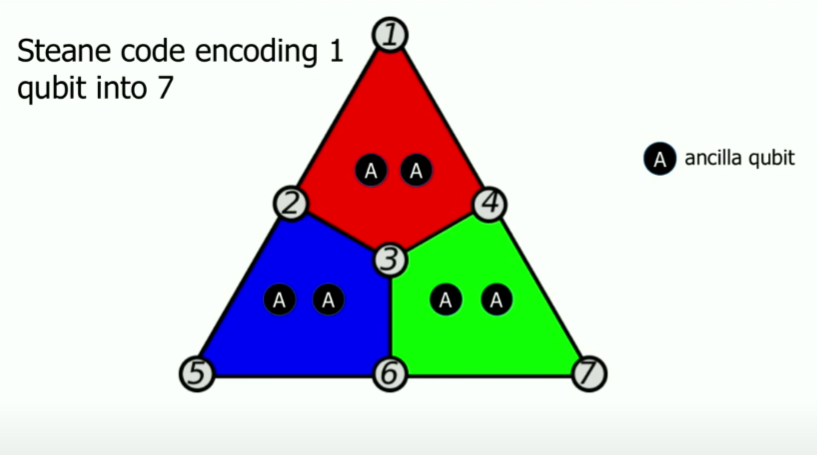
\includegraphics[width=0.75\linewidth]{img/Steane.png}
    \caption{Steane-Code}
    \label{fig:Steane}
\end{figure}

Um die Qubits zu überwachen werden zusätzliche Qubits benötigt, da das direkte Auslesen der daten Qubits den Quantenzustand zerstören würde.
Diese zusätzlichen Qubits werden als \textbf{Ancilla Qubit} bezeichnet und mit den eigentlichen Qubits verschränkt.\\

\textbf{Fehlertoleranz}\\
Diese Herangehensweise ist jedoch auch nicht perfekt. Die Ancilla Qubits sind gleichermaßen anfällig gegenüber Fehlern wie die eigentlichen Qubits.\\

\begin{figure}[H]
    \centering
    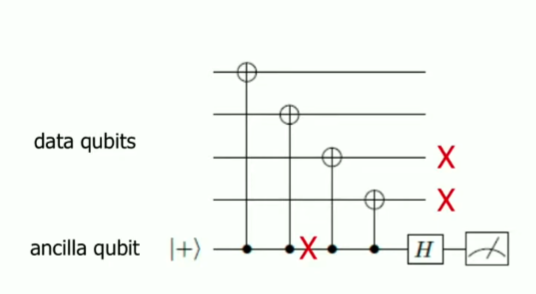
\includegraphics[width=0.75\linewidth]{img/Fehlertoleranz.png}
    \caption{Fehlertoleranz von Ancilla Qubits}
    \label{fig:Fehlertoleranz}
\end{figure}

Dieses Abbildung zeigt, wie ein einzelner Fehler in einem CNOT Gatter auf dem Ancilla Qubit Messung der Daten Qubits als Fehler kennzeichnet, obwohl diese nicht fehlerhaft sind.\\
Die Folge hieraus ist, dass die Fehlerkorrektur mit wenigen Qubits nicht ausreicht um diesen logischen Qubit vollkommen fehlerfrei zu halten.\\

Hierbei werden zwischen zwei Paritätchecks unterschieden. Ein $Z$ und $X$ Parität, welcher festlegt, ob der Fehler in den Ancilla Qubits CNOT Gattern oder den Daten Qubits aufgetreten ist.\\

\textbf{Suface Code}\\
Eine weitere Methode zur Fehlerkorrektur ist der Surface Code, welcher auf einem 2D Gitter von Qubits basiert.
Dieser Code ist in der Lage Fehler zu detektieren und zu korrigieren, solange die Fehlerdichte unter einem bestimmten Wert bleibt.\\

Die Größe des Surface Codes ist variabel und kann skaliert werden, um die Fehlerkorrektur zu verbessern.
Es gibt jedoch ein Threshold, an der die Vergößerung des Codes keine Verbesserung mehr bringt.
Durch die vorher besprochene Fehlertoleranz der Ancilla Qubits wird die Effektivität des Surface Codes gedeckelt.
Die Fehler in der Korrektur werden hierbei mehr, als wenn keine Korrektur vorgenommen wird und es würde keinen Sinn ergeben, den Surface Code weiter zu vergößern.\\

Die Nachfolgende Abbildung eines Surface Codes des Grades $d=3$ zeigt wie die Qubits in einem 2D Gitter angeordnet sind und wie die Fehlerkorrektur durchgeführt wird.
Jede Überschneidung des Gatters stellt ein physischen Qubit dar. Die Kreise in den Quadraten sind die Ancilla Qubits, welche die Fehlerkorrektur durchführen.\\

\begin{figure}[H]
    \centering
    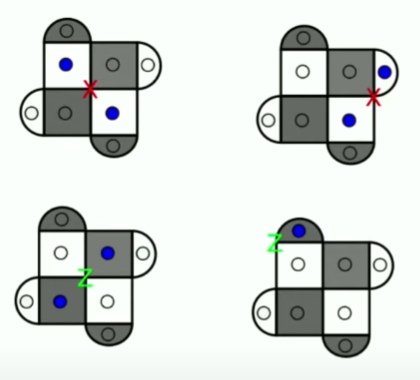
\includegraphics[width=0.6\linewidth]{img/Errors.png}
    \caption{Fehlerkorrektur durch Surface Code des Grades $d=3$}
    \label{fig:Surface-Code}
\end{figure}

Ancilla Qubits in einem weißen Feld prüfen die Qubits auf ein logisches $X$ und Ancilla Qubits in einem Schwarzen Feld prüfen die Qubits auf ein logisches $Z$.\\

Ancilla Qubits, die ein Fehler erkennen, werden als Blau markiert. Durch die Position dieser und für welche Daten Qubits diese zuständig sind wissen wir welche Qubits fehlerhaft sind.\\

\textbf{Praktische Umsetzung}\\
Am 09.12.2024 hat Google den ersten selbst korrigierenden Quantencomputer vorgestellt, der auf dem Surface Code basiert.
Der Chip namens \textbf{Willow} basiert auf 105 physischen Qubits, wobei diese auf der 7x7 Surface Code Architektur aufbaut.
Dies resultiert in 49 Qubits, die deutlich weniger anfällig gegen Fehler sind als phyische Qubits. Die restlichen Qubits werden für Parität und error Korrektur gebraucht.\\

\begin{figure}[H]
    \centering
    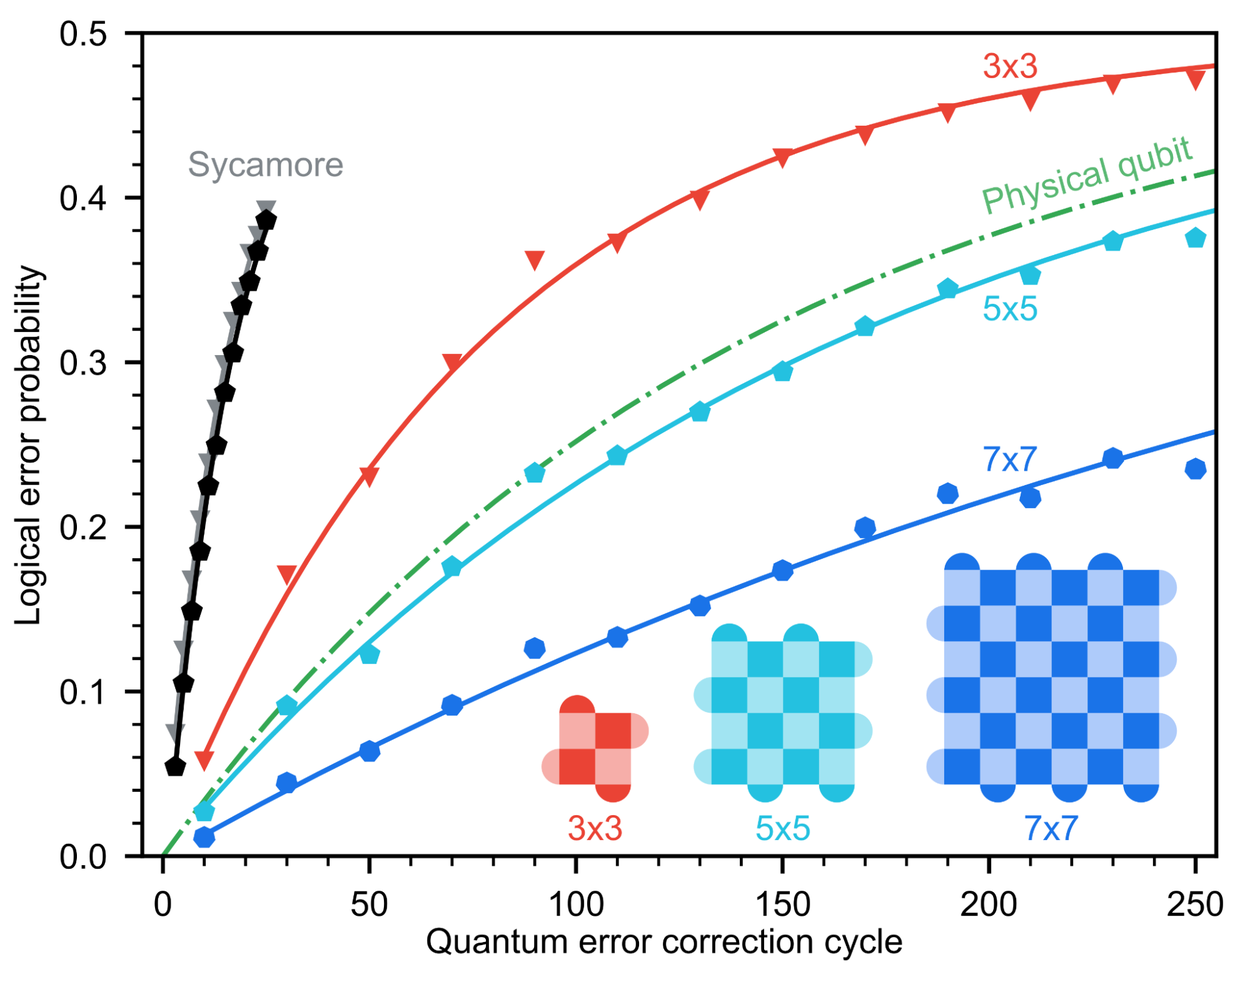
\includegraphics[width=0.7\linewidth]{img/Surface-Code-Scaling.png}
    \caption{Error Korrektur des 7x7 Surface Code}
    \label{fig:Willow}
\end{figure}

Außerdem wurde durch die Anwendung des Surface Codes die $T_1$ Zeit von $20\mu s$ auf $68\mu s\pm13\mu s$ erhöht und ermöglich hierdurch mehr Operationen pro Qubit.\\

\newpage 

\bibliographystyle{natdin}
	\bibliography{references} % expects file "references.bib"
	\addcontentsline{toc}{section}{References}
\end{document}
